\makeatletter
\renewcommand{\chapter}{%
  \if@openright\cleardoublepage\else\clearpage\fi % Remove quebra padrão
  \secdef{\@chapter}{\@schapter}}
\makeatother


\titleformat{\chapter}[hang]{\huge\bfseries}{\thechapter}{1em}{}
\titlespacing*{\chapter}{0pt}{*0}{20pt} % Ajusta espaçamentos antes/depois do capítulo

\chapter{Revisão Bibliográfica}

A renderização em tempo real tem evoluído significativamente no desenvolvimento de jogos digitais, abrangendo algoritmos de rasterização, técnicas de sombreamento e, mais recentemente, a introdução do \textit{ray tracing} em tempo real. Esta seção analisa os principais conceitos e avanços que moldaram o estado da arte na renderização em tempo real, destacando seu impacto no desempenho e na qualidade visual dos jogos.

\begin{figure}[h!]
    \centering
    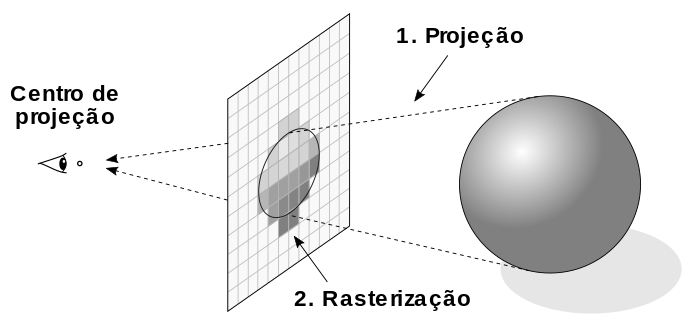
\includegraphics[width=0.7\textwidth]{04_rasterization.png}
    \label{fig:Rasterizaçao - Diagrama}
    
    \cite{RDiagram}
\end{figure}
\section{Rasterização}

A rasterização é a técnica predominante para a renderização em tempo real em jogos, devido à sua eficiência computacional. Este processo envolve a conversão de cenas tridimensionais em imagens bidimensionais, calculando a cor de cada pixel com base nos objetos visíveis na tela.\cite{RTR} a rasterização é especialmente adequada para aplicações que requerem altas taxas de quadros, como jogos, pois pode ser otimizada para ser executada diretamente no hardware das GPUs modernas.

Entretanto, a rasterização tem limitações na simulação de efeitos de iluminação complexos, como reflexos e refrações. Para contornar essas limitações, desenvolvedores utilizam técnicas complementares, como \textit{Screen Space Ambient Occlusion} (SSAO) e \textit{Screen Space Reflections} (SSR), que ajudam a simular oclusão de ambiente e reflexos de maneira mais convincente \cite{MCGuire:2011}.





\section{Ray Tracing em Tempo Real}

\begin{figure}
    \centering
    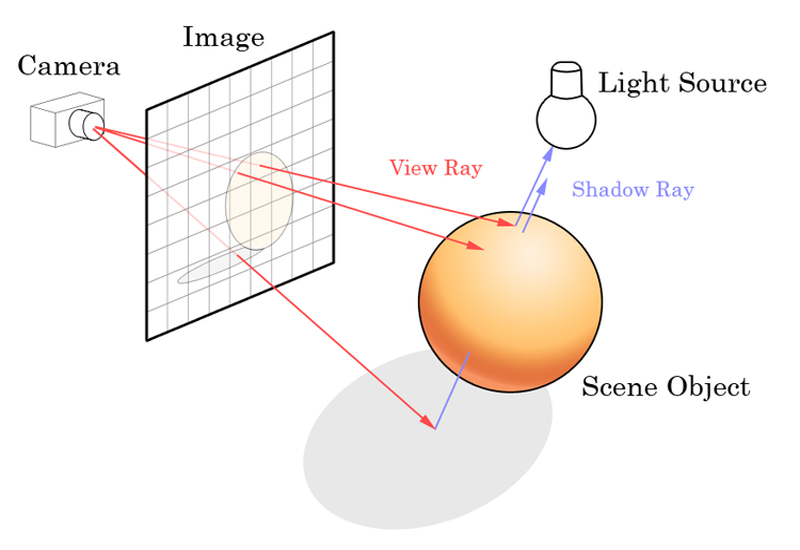
\includegraphics[width=0.5\linewidth]{Cara-Kerja-Ray-Tracing.jpg}
    \label{fig:RTX - Diagrama}
    
    \cite{RTDiagram}
\end{figure}

O \textit{ray tracing} em tempo real emergiu como uma das inovações mais significativas nos gráficos digitais. Diferente da rasterização, o \textit{ray tracing} simula com maior precisão a interação da luz com os objetos em uma cena, proporcionando reflexos, sombras e refrações mais realistas. Historicamente, o \textit{ray tracing} convencional era inviável para jogos devido ao seu alto custo computacional, sendo amplamente utilizado em filmes e animações pré-renderizadas \cite{PBR}



Com o advento de GPUs equipadas com núcleos dedicados ao \textit{ray tracing}, como as da arquitetura Turing da NVIDIA, essa técnica se tornou viável em tempo real, embora ainda com limitações de desempenho. Assim, em Hybrid Rendering for Real-Time Ray Tracing \cite{Barré-Brisebois2019}, uma solução híbrida que combina o ray tracing para efeitos específicos (como reflexos em superfícies metálicas) e a rasterização para o restante da cena tem se mostrado eficaz para equilibrar qualidade visual e desempenho. 
\\
\\
\\
\\
\\
\\\\\\\\

\section{Global Illumination}

\begin{figure}
    \centering
    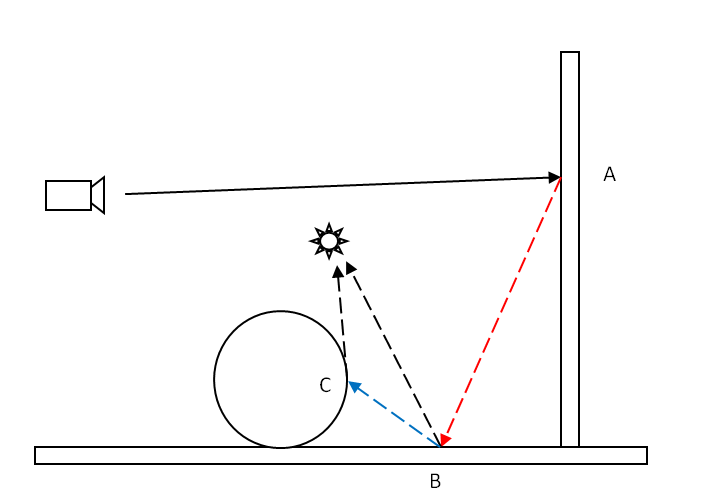
\includegraphics[width=0.45\linewidth]{GI.png}
    \label{fig:RTX - Diagrama}

    \cite{GIDiagram}
\end{figure}

Um conceito essencial na renderização em tempo real é o de \textit{Global Illumination} (GI), que trata da interação indireta da luz em uma cena, simulando múltiplas reflexões e criando ambientes mais realistas. \cite{Dachsbacher2005} discutem a técnica conhecida como \textit{Reflective Shadow Maps} (RSM), que aproxima a iluminação indireta com base em mapas de sombras refletidas.

Entretanto, as técnicas de GI podem ser computacionalmente exigentes, representando um desafio significativo para a renderização em tempo real. Abordagens como \textit{pre-computed radiance transfer} (PRT) e mapas de iluminação são utilizadas para aliviar parte desse custo, permitindo que a iluminação de cenas estáticas seja precalculada, como discutido por \cite{IR:1997}.

\section{Otimização de Desempenho}

Um dos principais desafios na renderização em tempo real é otimizar o desempenho sem comprometer a qualidade visual. Para garantir uma experiência de jogo fluida, técnicas como \textit{Level of Detail} (LoD) e \textit{frustum culling} são amplamente utilizadas. O LoD ajusta a complexidade dos objetos de acordo com sua proximidade à câmera, enquanto o \textit{frustum culling} elimina objetos não visíveis na cena, reduzindo a carga de processamento \cite{LoD}.

As arquiteturas de GPUs multicore desempenham um papel crucial ao permitir o paralelismo em larga escala, fundamental para atender às crescentes demandas gráficas dos jogos \cite{SIEGEL19873}. Além disso, a integração de técnicas de \textit{machine learning} e a exploração de renderização baseada em nuvem (\textit{cloud gaming}) emergem como tópicos promissores, com o potencial de melhorar ainda mais o desempenho gráfico em jogos futuros \cite{Keller2018}.

\section{Conclusão}

A revisão bibliográfica revela que a renderização em tempo real é um campo dinâmico, impulsionado por avanços em hardware e algoritmos. O \textit{ray tracing} em tempo real destaca-se como uma técnica inovadora, embora enfrente desafios de desempenho que precisam ser superados. Técnicas de otimização como LoD, SSAO, SSR, juntamente com GPUs de última geração, são essenciais para equilibrar qualidade visual e taxa de quadros, um fator crítico para a experiência de jogo. O futuro dessa área promete soluções ainda mais sofisticadas, incluindo a aplicação de inteligência artificial na renderização e o desenvolvimento de tecnologias de renderização baseadas em nuvem.